\chapter{Umsetzung in RoboCup2D}
    % ``Was ist RoboCup'' \\
    % ``Was für Ligen gibt es'' \\
    % ``Was für eine Domäne ist es im Vergleich zu anderen'' \\
    % \\
    RoboCup ist ein Fußball Simulator, der seine Anfänge in 1993 in Japan, Tokyo gefunden hat. Eine Gruppe von Forschern, inklusive Minoru Asada, Yasuo Kuniyoshi und Hiroaki Kitano, haben als einen Wettbewerb unter dem Namen \textbf{Robot J-League} gestartet. Der Name stammt von einer professionellen japanischen Fußball Liga.\\
    \\
    Nach einem Monat haben sie jedoch weltweit überwältigendes Feedback bekommen und haben die Initiative als internationales Projekt weitergeführt, daher kam die Umbenennung zur \textbf{Robot World Cup Initiative}, kurz RoboCup. \\
    % \textit {(source: http://www.robocup.org/about-robocup/a-brief-history-of-robocup/)} \\
    \\
    Die RoboCup Initiative hat betreibt derzeit sechs große Wettbewerbe, die sich jeweils wieder in Ligen und Subligen aufteilen lassen. Darunter fällt \textbf{RoboCup Soccer}, \textbf{RoboCup Rescue Rescue}, \textbf{RoboCup Junior}, \textbf{RoboCup Logistics}, \textbf{RoboCup @ Work} und \textbf{RoboCup @ Home}. Unsere Implementierung fällt in die Subliga \textbf{2D Soccer Simulation}, in der es darum geht in einer zweidimensionalen Welt zwei Fußballmannschaften gegeneinander antreten zu lassen.\\
    \\
    Die Aufgabe die wir angehen gehört zu einem Fragement von RoboCup2D, genannt \textbf{Half Field Offense}.\\

    \begin{figure}[htbp]
        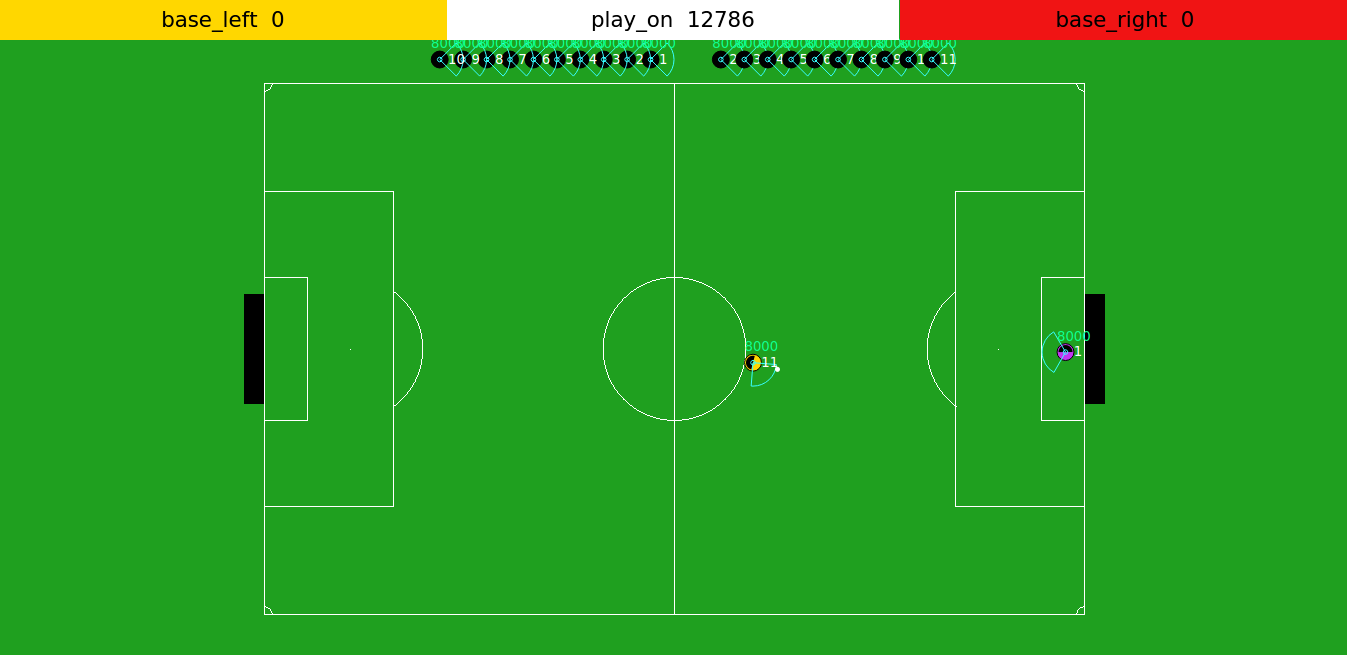
\includegraphics[width = 1.0\textwidth, center]{../pictures/full-field.png}
        \caption{Screenshot von dem gesamten Spielfeld von RoboCup2D \label{fig:somelabel}}
    \end{figure}

    \section{Half Field Offense}

        Die Domäne Half Field Offense grenzt das Spielfeld auf eine Hälfte ein, sodass wir 4 Angreifer und 3 Verteidiger + Torwart haben. Diese Einschränkung vereinfacht den Such- und Zustandsraum immens und erlaubt potenziell eine Wiederverwendbarkeit der Agenten, wenn eine vollständige Mannschaft aufgebaut wird.\\
        \\
        In unserer Implementierung haben wir lediglich ein 1vs1 Szenario, also ein Angreifer gegen ein Torwart. Diese sieht jedoch explizit ein nahtlosen Skalierung auf ein 4vs4 Szenario vor, sodass weitere Parametrisierung ohne viel Aufwand ausprobiert werden können.\\

        \begin{figure}[htbp]
            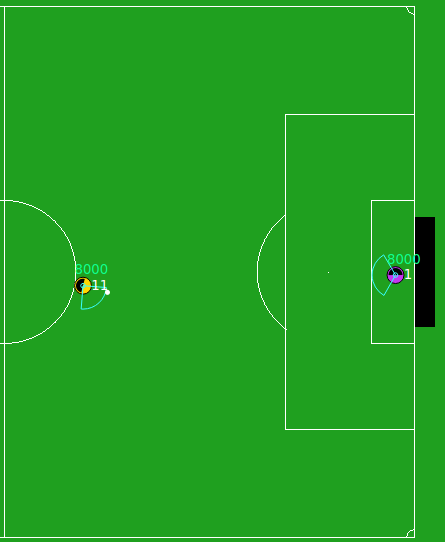
\includegraphics[width = 0.5\textwidth,height = 0.4\textheight, center]{../pictures/half-field.png}
            \caption{Screenshot von dem Spielfeld für den Subtask HFO \label{fig:somelabel}}
        \end{figure}
        \noindent
        Im Folgenden wird die Domäne samt Zustandsraum und Aktionen erklärt, sowie ihren Einschränkungen für die Anwendung von Machine Learning Algorithmen.\\
        % \cite{ http://www.cs.utexas.edu/users/ai-lab/?hausknecht:aamasws16 }
\newpage
        \subsection{Zustandsraum}
            % ``Unterschiedliche Zustandsräume, kommt drauf an wie viele Spieler aufm Feld sind (zitat vom HFO Paper)''\\
            % ``Angepasst für Maschinen (zitat HFO)'' \\
            % ``Umrechnung für Menschen'' \\
            % ``Fullstate flag''
            Der Zustandsraum der HFO Domäne kann in den \textbf{High Level State} und den \textbf{Low Level State} aufgeteilt werden. Der Unterschied ist lediglich in der Dimensionalität, da man aus dem Low Level State den High Level State ableiten kann. Die Zustandsräume werden durch folgende Formeln definiert:\\
            
            \begin{mdframed}
            \textit{Sei T die Anzahl der Teammitglieder, O die Anzahl der Gegner:}
            \begin{center}
                \textit{High Level State} $ := 10 + 6T + 3O \hspace{10mm} $ \\
                \textit{Low Level State}  $ := 58 + 8T + 8O \hspace{9mm} $ \\
            \end{center}
            \end{mdframed}
%            \textit{(Frage: Alles vom Paper abschreiben oder referenzieren?)} \\
 %           \\
            In unserem 1vs1 High Level Setting haben wir damit 13 Zustandsparameter. Vier von diesen Parametern gehören zu dem Torwart, aber da seine Position implizit durch andere Ausprägungen gegeben ist, beachten wir sie nicht. Redundante Information würde den Suchraum unnötig aufblähen und die Suche verlängern. Deshalb wurden nur die folgenden 9 Zustände bereitgestellt:

            \begin{table}[H]
                \begin{center}
                \hspace*{-2cm}
                \begin{tabular}{ |l|c|c|c|c|c| } 
                    \hline
                    \hfill Zustandsbeschreibung                          & Wertebereich & Winkel & Boole'sch & Lage & Anderes \\ \hline
                    x-Koordinaten                                        & $[ -1, +1 ]$ & \hfill & \hfill    &      & X       \\ \hline
                    y-Koordinaten                                        & $[ -1, +1 ]$ & \hfill & \hfill    &      & X       \\ \hline
                    Sichtrichtung                                        & $[ -1, +1 ]$ & X      & \hfill    &      & \hfill  \\ \hline
                    Nähe zum Ball                                        & $[ -1, +1 ]$ & \hfill & \hfill    & X    & \hfill  \\ \hline
                    Winkel zum Ball                                      & $[ -1, +1 ]$ & X      & \hfill    &      & \hfill  \\ \hline
                    Kann eine Ballaktion ausgeführt werden               & $[ -1, +1 ]$ & \hfill & X         &      & \hfill  \\ \hline
                    Winkel zum Mittelpunkt des Tors                      & $[ -1, +1 ]$ & X      & \hfill    &      & \hfill  \\ \hline
                    Größte offene Winkel zwischen Torwart und Torpfosten & $[ -1, +1 ]$ & X      & \hfill    &      & \hfill  \\ \hline
                \end{tabular}
                \end{center}
                \caption{Zustandsraum von HFO 1vs1 \label{fig:somelabel}}
            \end{table}

            % \hspace*{-1.5cm}
            % \textit{(Muss hier eine Erklärung wie der Zustand kodiert war hin, also Normalisierung der Winkel?\\
            % \hspace*{-1.5cm} Wäre dann eigentlich abschreiben ab 15.1.1 von https://github.com/LARG/HFO/blob/master/doc/manual.pdf)}
            % (src: https://github.com/LARG/HFO/blob/master/doc/manual.pdf ab 15.1.1)
            \noindent
            Der Zustand kann in 4 Kategorieren unterteilt werden, die auf den Wertebereich von $[ -1, +1 ]$ reduziert wurden.

            \subsubsection*{Winkelkodierung}
                Die Winkel sind im Bereich von $[0, \pi]$ und durch folgende Formel auf den Bereich $[-1, +1]$ transformiert:

                \begin{mdframed}
                    Sei $f : [0,\pi] \rightarrow [-1, +1]$ die Kodierungsfunktion \\
                    \hspace*{5mm} $g : [-1, +1] \rightarrow [0, \pi]$, die Inverse: \\[4mm]
                    \hspace*{10mm} \Resize{4.5cm}{$f(x) = (\frac{x}{\pi} - 1) \cdot 2$}
                    \hspace*{20mm} \Resize{4.5cm}{$g(x) = (\frac{x}{2} + 1) \cdot \pi$}
                \end{mdframed}

            \subsubsection*{Boole'sche Kodierung}
                Die boole'schen Werte sind binär und $-1$ entspricht $false$ und $1$ entsprechend $true$.

            \subsubsection*{Lagekodierung}
                Die Lagekodierung ist normalisiert auf der maximale diagonale Länge des Spielfelds die durch $max_{l} = \sqrt{l^2 + w^2}$ gegeben ist, wobei $l$ die Länge und $w$ die Breite ist. In dem Fall für HFO, entspricht sie $sqrt(2^2 + 2^2) ~= 2.82$.\\

                \begin{mdframed}
                Sei $f : [-max_{l}, max_{l}] \rightarrow [-1, +1]$ die Kodierungsfunktion \\
                    \hspace*{5mm} $g : [-1, +1] \rightarrow [-max_{l}, max_{l}]$, die Inverse: \\[4mm]
                    \hspace*{25mm} \Resize{3.5cm}{$f(x) = \frac{x}{max_{l}}$}
                    \hspace*{20mm} \Resize{3.5cm}{$g(x) = x \cdot max_{l}$}
                \end{mdframed}

            \subsubsection*{Anderes}
                Unter diese Kategorie fallen nur die x- und y-Koordinaten und sind trivialerweise im Bereich von [-1, +1], weil das die Grenzen des Spielfelds sind.

            \hfill \\[2mm]
            \noindent
            Wir wollen an dieser Stelle anmerken dass wir alle Zustände mit normal verteilten Rauschen empfangen haben.
        \subsection{Aktionsraum}
            % ``Gibt 6 nicht parametrisierte Aktionen, die wir benutzt haben''\\
            % ``Gibt noch andere parametrisierte''
            Es gibt 8 parametrisierte und 6 nicht parametrisierte Aktionen. Wir haben die Algorithmen über 5 der 6 Aktionen ohne zusätzlichen Argumente trainiert. Die Aktion \textit{CATCH} ist für Angreifer illegal und wurde deshalb weggelassen. Die folgende Aufzählung beschreibt alle Aktionen:
            \textit{(Genauere Erklärung von benutzen Aktionen kommt noch)}

            \begin{multicols}{2}
                \textbf{Parametrisierte}
                \begin{itemize}
                    \item Dash(power, degrees)
                    \item Turn(degrees)
                    \item Tackle(degrees)
                    \item Kick(power, degrees)
                    \item Kick\_To(x-coords, y-coords, speed)
                    \item Move\_To(x-coords, y-coords)
                    \item Dribble\_To(x-coords, y-coords)
                \end{itemize}
                \textbf{Nicht parametrisierte}
                \begin{itemize}
                    \item Move
                    \item Shoot
                    \item Dribble
                    \item Intercept
                    \item Catch
                    \item No-Op
                \end{itemize}
            \end{multicols}
            \noindent
            Jedes Spiel hatte eine maximale Zeit die in Frames aufgeteilt war und jeder Agent wird zu jedem Frame gefragt ob er eine neue Aktion ausführen will. Wenn ein Timeout von einem festen Zeitabstand kommt, wird pauschal die No-Op Aktion ausgeführt.

        \subsection{Einschränkungen}
            % ``Sparse Fitness''                 \\
            % ``Simulation Learning''            \\
            % ``Hochdimensional Kontinuierlich'' \\
            % ``Auch genannt Black Box RL''
            Diese Domäne hat viele Einschränkungen wenn man sie mit herkömmlichen Machine Learning Tasks vergleicht \textit{(Vergleich Moonrover, Roboterarm etc.)}. Zum einen erlaubt sie uns wegen der Implementierung nicht in die Zukunft zu propagieren und zu schauen wie gut eine Entscheidung ist. Wir haben eine Simulation die erst nachdem ein Spiel fertig ist ein Fitnesssignal sendet und wir daraufhin abzuleiten müssen ob die lange Aktionsketten die wir ausgeführt haben uns zum Erfolg führten. Diese Eigenschaft nennt sich \textbf{sparse Fitness} und findet sich in Beispielen wie \textit{(Zitat)}

            \begin{center} \textit{(Simulation based learning)} \end{center}
            \begin{center} \textit{(Kontinuierlicher Zustandsraum, hohe Abstraktion)} \end{center}
            % (cite https://gym.openai.com/docs/rl#black-box-optimization-and-the-cross-entropy-method)

    \section{Implementierung der Algorithmen}
        % ``Server in Haskell, HFOServer in C++, Agenten in Python''
        Der ausführliche Aufbau der Algorithmen wird näher im Appendix erklärt, hier schauen wir uns die Parametrisierung grobe Funktionsweise an. Die Simulation kann in die folgenden drei Teile unterteilt werden.

        \subsubsection*{Simulationsserver}
        Der Simulationsserver ist in C++ geschrieben und wurde 1-zu-1 aus \cite{hfo} übernommen. Er wird durch Flags beim Starten parametrisiert.
        % (src: https://github.com/LARG/HFO)

        \subsubsection*{Agenten}
        Die Agenten sind in Python geschrieben und stellen eine Erweiterung von einem der Beispielskripte dar\cite{hfo}. Diese Prozesse werden auch mit eigenen Kommandozeilenparametern aufgerufen.

        \subsubsection*{Koordinator}
        Der Koordinator ist für die Umsetzung des GAs und den jeweiligen Kodierungen zuständig, startet den Server und die Agenten Skripte und überwacht die Simulation. Er ist, wie alle folgenden Codebeispiele, in Haskell geschrieben.

        \subsubsection*{Simulation}
        Jedes Team hat pro Generation 25 Spiele gespielt und die gesamte Simulation bestand aus insgesamt 375000 Spielen.
        Die Episodenzeit wurde auf 500 Echtzeitsekunden beschränkt, da ansonsten die simulierte Zeit pro Spiel nicht praktikabel war. \\

        \noindent
        Für alle Simulationen galten die folgenden Rahmenbedingungen:

        \begin{center}
            \begin{tabular}{ |c|c| } 
                \hline
                Generationen       & $300$  \\ \hline
                Populationsgröße   & $50$   \\ \hline
                Teamepisoden       & $25$   \\ \hline
                Episodenzeit       & $500s$ \\ \hline
                Ball nicht berührt & $50s$  \\ \hline
                $\alpha$           & 0.25   \\ \hline
                $\beta$            & 0.10   \\ \hline
            \end{tabular}
        \end{center}

        \subsection{Wahrscheinlichkeitsverteilung von Aktionen}

            Der erste Algorithmus hat als Kodierung der Individuen eine diskrete Wahrscheinlichkeitsverteilung über 5 Aktionen benutzt. Wenn der Agent gestartet wurde samplet er jeden Zeitschritt ohne Wissen über jeglichen Zustand aus dieser Verteilung raus.

            \subsubsection*{Kodierung}

            \begin{figure}[H]
                \begin{mdframed}
                    Sei das Set von allen Aktionen $ X := $ \{Move, Shoot, Dribble, Intercept, No-Op\}, \\
                    $P(x)$ die Wahrscheinlichkeit dass $x$ eintrifft, dann gilt: \\[2mm]
                    \hspace*{25mm} \Resize{8cm}{$\forall x \in X: P(x) \geq 0 \;\;\land\;\; \sum_{x \in X}^{} P(x) = 1$}
                \end{mdframed}
                \caption{\label{kodierung} Kodierung der Aktionen als Wahrscheinlichkeitsverteilung}
            \end{figure}

            \subsubsection*{Kreuzung}
            Die Kreuzung wurde auf zwei verschieden Arten umgesetzt, wobei sie im Vergleich an der vollständige Simulation weder neueartige Lösungen entwickelt haben, noch die Konvergenzzeit beeinflusst wurde.

            \subsubsection*{Generator}
            Die erste Methode kam aus der Idee wie man mit einer absehbaren Laufzeit eine Wahrscheinlichkeitsverteilung über $n$ Aktionen erstellt. Dafür werden $n-1$ zufällige Zahlen erstellt, als Liste verpackt, sortiert und jeweils eine $0$ von vorne und eine $100$ am Ende angehängt.

            \begin{mdframed}
            \begin{minted}[escapeinside=||, linenos]{haskell}
> let n = 5
> take (n-1) <$> getRandomRs (0,100)
[87, 15, 55, 38]
> sort it
[15, 38, 55, 87]
> 0 : it ++ [100]
[0, 15, 38, 55, 87, 100]
            \end{minted}
            \end{mdframed}
            \noindent
            Anschließend wird diese Liste dupliziert und um ein Element nach rechts verschoben und paarweise voneinander abgezogen.
            \begin{mdframed}
            \begin{minted}[escapeinside=||, linenos]{haskell}
> let l1 = [0, 15, 38, 55, 87, 100]
> drop 1 l1
[15,38,55,87,100]
> let l2 = it
> {-
  [15, 38, 55, 87, 100]
- [ 0, 15, 38, 55,  87, 100]
= [15, 23, 17, 32,  13]
-}
> zipWith (-) l2 l1
[15, 23, 17, 32, 13]
> sum it
100
            \end{minted}
            \end{mdframed}
            \noindent
            Damit haben wir eine Wahrscheinlichkeitsverteilung über 5 Aktionen und können uns sicher sein dass sie aufsummiert immer $100$ ergibt. Die Kreuzung von zwei solcher Individuen wurde mit den jeweiligen Listen umgesetzt, aus denen sie generiert wurden. Dafür wurde elementweise der Durchschnitt berechnet und daraus entsteht dann eine neue Generatorliste aus der sich die Verteilung berechnen lässt.
            \begin{mdframed}
            \begin{minted}[escapeinside=||, linenos]{haskell}
> let individualA = [0, 15, 38, 55, 87, 100]
> let individualB = [0, 7, 22, 35, 51, 100]
> zipWith (\x y -> (x + y) `div` 2) individualA individualB
[0, 11, 30, 45, 69, 100]
            \end{minted}
            \end{mdframed}
            \subsubsection*{Normalisierung}
            Die zweite Methode hat beide Verteilungen genommen, die Wahrscheinlichkeiten für jeweiligen Aktionen addiert und folgendermaßen normalisiert.\\
            \noindent
            \begin{figure}[H]
                \begin{mdframed}
                    Seien $\mathcal{A, B}$ die diskreten Wahrscheinlichkeitsverteilungen, $l = |\mathcal{A}|$:\\[4mm]
                    \hspace*{40mm}\Resize{6.5cm}{$\mathcal{C} := \{ \frac{(a_i + b_i)}{l} \; | \; a_i \in \mathcal{A}, b_i \in \mathcal{B}\}$} \\[4mm]
                    dann ist $\mathcal{C}$ ist ihre Verknüpfung.
                \end{mdframed}
                \caption{\label{norm-prop} Normalisierung von Wahrscheinlichkeitsverteilungen}
            \end{figure}

            \subsubsection*{Mutation}
            Die Mutation wurde auch mit jeweils dem Generator sowie Normalisierung umgesetzt. Im Kern ist jedoch die Funktion die das $\delta$ benutzt und es mit zufälligen Vorteichen in die Anzahl der Aktionen aufgeteilt. Man kann sich das $\delta$ als Veränderungsfaktor vorstellen, je höher er ist, umso unterschiedlicher wird die Wahrscheinlichkeitsverteilung.
            \begin{mdframed}
            \begin{multicols}{2}
                \begin{minted}[escapeinside=||, linenos]{haskell}
> let delta = 20
> splitDelta delta 5
[-4, +4, +4, -4, -4]
                \end{minted}
                \begin{minted}[escapeinside=||]{haskell}
> let delta = 100
> splitDelta delta 4
[-25, +25, +25, -25]
                \end{minted}
            \end{multicols}
            \end{mdframed}
            \subsubsection*{Generator}

            Wir erstellen teilen das $\delta$ in $n-1$ Teile auf, fügen eine $0$ von vorne und $100$ von hinten hinzu und verknüpfen es analog wie in der Kreuzung mit dem Ausgangsgenerator. Diesmal müssen wir jedoch die Zahlen per Hand auf den Bereich von $0 - 100$ begrenzen.
            \begin{mdframed}
            \begin{minted}[escapeinside=||, linenos]{haskell}
> let delta = 100
> splitDelta delta 4
[-25, +25, +25, -25]
> let mutGen = 0 : it ++ [100]
> let child = [0, 14, 31, 49, 75, 100]
> {-
  [0, -25, +25, +25, -25, 100]
+ [0,  14,  31,  49,  75, 100]
= [0, -11,  56,  74,  50, 200]
min 0
  [0,   0,  56,  74,  50, 200]
max 100
  [0,   0,  56,  74,  50, 100]
sort
  [0,   0,  50,  56,  74, 100]
-}
> sort $ zipWith (((max 0 . min 100) .) . (+)) child mutGen
[0,0,50,56,74,100]
            \end{minted}
            \end{mdframed}

            Aus diesem Generator kann wieder eine Wahrscheinlichkeitsverteilung erstellt werden.

            \subsubsection*{Normalisierung}

            Bei der Lösung mit der Normalisierung generieren wir uns wieder die Liste aus dem $\delta$, summieren sie elementweise mit der Verteilung, überprüfen ob die Grenzen von $[0,100]$ überschritten wurden und normalisieren sie wie in der Kreuzung.
            \begin{mdframed}
            \begin{minted}[escapeinside=||, linenos]{haskell}
> let delta = 50
> splitDelta delta 5
[-10, +10, +10, -10, -10]
> let mutGen = it
> let child = [15, 8, 34, 21, 22]
> zipWith (((max 0 . min 100) .) . (+)) child mutGen
[5,18,44,11,12]
> normalizeDist it
[5,20,48,12,15]
            \end{minted}
            \end{mdframed}
            Damit bekommen wir wieder eine veränderte diskrete Verteilung zurück.
        \subsection{Cross Entropy mit DCT}
            1108 Gewichte für das 9-12-5 LSTM Netz in 20 Koeffizienten kodiert (1:55)
        \subsection{Neuroevolution mit DCT}
            1108 Gewichte für das 9-12-5 LSTM Netz in 20 Koeffizienten kodiert (1:55)
        \subsection{CoSyNE mit DCT}
            1108 Gewichte für das 9-12-5 LSTM Netz in 20 Koeffizienten kodiert (1:55)

    \section{Resultate}
        Im folgenden Teil beschreiben wir die Resultate und versuchen diese zu begründen. Durchschnittlich hat eine Trainigsphase mit 300 Generationen, Population der Größe 50 und 25 Episoden pro Team 30 Stunden gedauert. Der Suchraum für die Neuroevolution wurde von 916 Gewichten auf 20 Koeffizienten reduziert, welches einer Kompressionsrate 1:45 entspricht. Die Simulationen wurden auf einem Laptop mit einem Intel i5 mit Dual Core 2.9GHz und 4GB Arbeitsspeicher ausgeführt.\\[2mm]
        \noindent
        Nachdem wir pro Algorithmus die besten 5 Individuen ermittelt haben, ließen wir sie jeweils 10000 Spiele spielen, um die erfasste Fitness auf ihre Stabilität zu testen. \\[2mm]
        \noindent
        Sei $F_{Entwicklung}$ die entwickelte Fitness und $F_{Test}$ die neu getestete Fitness. Die Stabilität wird danach gemessen wie gering die Abweichung von $F_{Test}$ zu $F_{Entwicklung}$ ist. Je kleiner die Abweichung, umso stabiler und sicherer spielt das Individuum.\\

        \begin{mdframed}
        \begin{center}
            \hspace*{0mm} \Resize{6cm}{$\text{Abweichung} = \frac{F_{Entwicklung} - F_{Test}}{F_{Entwicklung}}$}
        \end{center}
        \end{mdframed}

        \subsection{1v1}
            Unser Lernziel für die HFO Domäne war einen offensiven Spieler zu trainieren der gegen einen vom Server gesteuerten Torwart so gut es geht Tore schießt. Das haben wir mit vier in Kapitel 2 angesprochenend Algorithmen getestet und stellen die Resultate vor. 

\newpage
            \subsubsection*{Wahrscheinlichkeitsverteilung}
                \begin{multicols}{2}
                    \noindent
                    Die Wahrscheinlichkeitsverteilung war der erste naive Ansatz um zu überprüfen ob die Domäne bereits durch eine einfache Kodierung lösbar ist. Leider ging die Varianz in der Population nach der $10$ Generation gegen $0$ und die Verteilung sah folgendermaßen aus:
                    \begin{table}[H]
                        \begin{center}
                        \begin{tabular}{ |l|r| } 
                            \hline
                            \hfill Aktionen & P(Aktion)  \\ \hline
                            Move      & 22\% \\ \hline
                            Dribble   & 22\% \\ \hline
                            Intercept & 22\% \\ \hline
                            No-Op     & 22\% \\ \hline
                            Shoot     &  2\% \\ \hline
                        \end{tabular}
                        \end{center}
                    \end{table}

                    \begin{figure}[H]
                        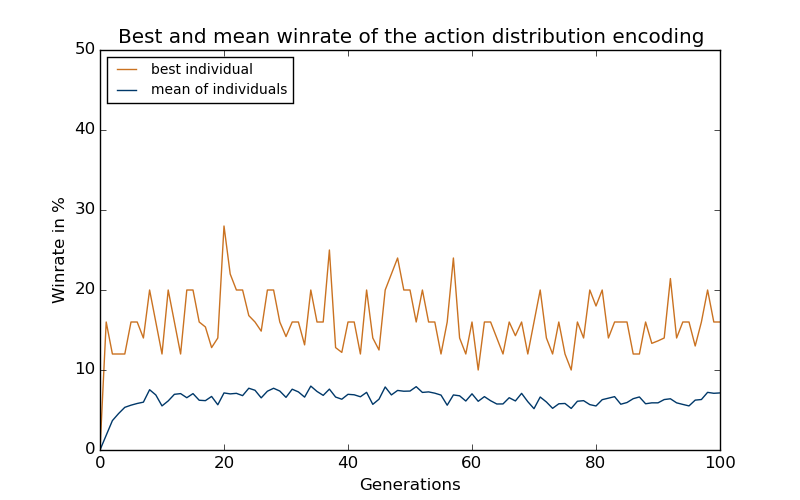
\includegraphics[scale=0.5]{../pictures/summary/actiondist-fitness.png}\\
                        \caption{Fitness Graph für die \\Wahrscheinlichkeitsverteilung}\label{fig:graph-ac}
                    \end{figure}
                \end{multicols}
                \noindent
                Die gesamte Population ist zu dem Ergebnis konvergiert, dass jede Aktion gleich wahrscheinlich ist, bis auf \textit{Shoot}. Die Schussaktion hat wahrscheinlich zu oft zu einem Schuss ins Aus geführt, was sofort das Spiel als zu Gunsten des Torwarts beendet.\\

                \noindent
                Die maximale erreichte Fitness beträgt 33\% und schwankt im Bereich von $[15,25]$ mit ein paar Ausreißern. Leider stellt sich heraus dass die besten drei Werte Ausreißer waren und keinesfalls die durchschnittliche Gewinnwahrscheinlichkeit darstellen. 

                \begin{table}[H]
                    \begin{center}
                    \begin{tabular}{ |l|r|r|r| } 
                        \hline
                        \hfill & Trained Fitness   & Tested Fitness   &          Error    \\ \hline
                          Nr.1 &          33.33\%  &          5.26\%  &          82.22\%  \\  
                          Nr.2 &          29.41\%  &          8.87\%  &          70.52\%  \\  
                          Nr.3 &          28.00\%  &          6.06\%  &          78.36\%  \\ 
                          Nr.4 &          25.00\%  &          2.18\%  &          91.28\%  \\ 
                          Nr.5 &          24.00\%  &          6.42\%  &          73.25\%  \\ \hline
                          Mean &  \textbf{27.95\%} &  \textbf{5.72\%}  & \textbf{79.53\%} \\ \hline
                    \end{tabular}
                    \end{center}
                    \caption{Stabilität der besten 5 Wahrscheinlichkeitsverteilungs Individuen \label{fig:actiondisttable}}
                \end{table}
                \noindent
                Die durchschnittliche Gewinnwahrscheinlichkeit liegt bei 5.72\% und wenn man den Spieler beobachtet kann man sich beim besten Willen nicht erklären, wie er überhaupt schafft Tore zu schießen, da er meistens versucht ins Tor zu laufen während ihm der Ball abgenommen wird. Es ist aber auch nicht verwunderlich, da der Spieler weder weiß wo der Torwart ist, ob er den Ball hat, noch wo er sich auf dem Spielfeld befindet. \\

                \begin{center} \textit{(Link zum Video)} \end{center}

\newpage
            \subsubsection*{Cross Entropy}
%                ``Graph zeigen, Interpretation bzw. Erklärung''
%                ``Aggressivität''
%                ``Nach ~ 50 Episoden stagniert''
                \begin{multicols}{2}
                    \noindent
                    \\[5mm]
                    Die Cross Entropy Methode hat sehr interessante Ergebnisse produziert, da sie durchschnittlich eine 4\% bessere Fitness hat, die Stabilität jedoch um 3\% schlechter ist, als wie die Wahrscheinlichkeitsverteilung.\\[2mm]
                    Sie ist nach ungefähr 50 Generationen konvergiert und die maximale erreichte Fitness beträgt 32\% und schwankt im Bereich von $[15,30]$. 
                    \begin{figure}[H]
                       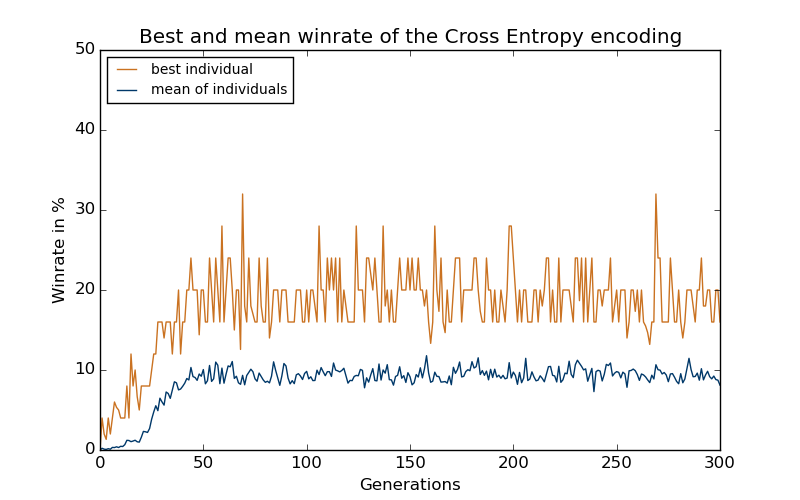
\includegraphics[scale=0.5]{../pictures/summary/cross-entropy-fitness.png}
                       \caption{Fitness Graph für Cross Entropy}\label{fig:graph-ce}
                    \end{figure}
                \end{multicols}

                \begin{table}[H]
                    \begin{center}
                    \begin{tabular}{ |l|r|r|r| } 
                        \hline
                        \hfill & Trained Fitness   & Tested Fitness  &          Error    \\ \hline
                          Nr.1 &          32.00\%  &          7.26\% &          77.31\%  \\  
                          Nr.2 &          32.00\%  &          7.46\% &          76.69\%  \\  
                          Nr.3 &          28.00\%  &          7.37\% &          73.68\%  \\ 
                          Nr.4 &          28.00\%  &          7.27\% &          74.04\%  \\ 
                          Nr.5 &          28.00\%  &          3.46\% &          87.64\%  \\ \hline
                          Mean &  \textbf{29.60\%} & \textbf{6.56\%} & \textbf{77.87\%}  \\ \hline
                    \end{tabular}
                    \end{center}
                    \caption{Stabilität der besten 5 Cross Entropy Individuen \label{fig:crossentropytable}}
                \end{table}
                \noindent
                Von den Werten sieht man kaum einen Unterschied zu der Wahrscheinlichkeitsverteilung, aber in der Simulation merkt man ein extrem aggressives Verhalten vom Spieler. Der Agent schießt den Ball sehr oft und versucht bereits nachdem er die Mitte des Spielfeldes überquert hat ein Tor zu schießen, unabhängig davon ob er in einer guten Position ist. Das führt natürlich wieder dazu dass er öfter ins Aus schießt, ist aber wesentlich interessanter anzuschauen, da er von Spiel zu Spiel unberechenbar ist. \\

                \begin{center} \textit{(Link zum Video}) \end{center}
\newpage
            \subsubsection*{Neuroevolution}
                \begin{multicols}{2}
                    \noindent
                    \\[5mm]
                    Der Ansatz die Gewichte naiv als DCT Koeffizienten darzustellen führe zu den besten Ergebnissen. Das stärkste Individuum hat knapp jedes zweite Spiel gewonnen und ist mehr als 3-mal stabiler als die Cross-Entropy Lösung. Die Fitness hat sich nach ungefähr 150 Generationen im Bereich von $[30,45]$ eingependelt.
                    \begin{figure}[H]
                       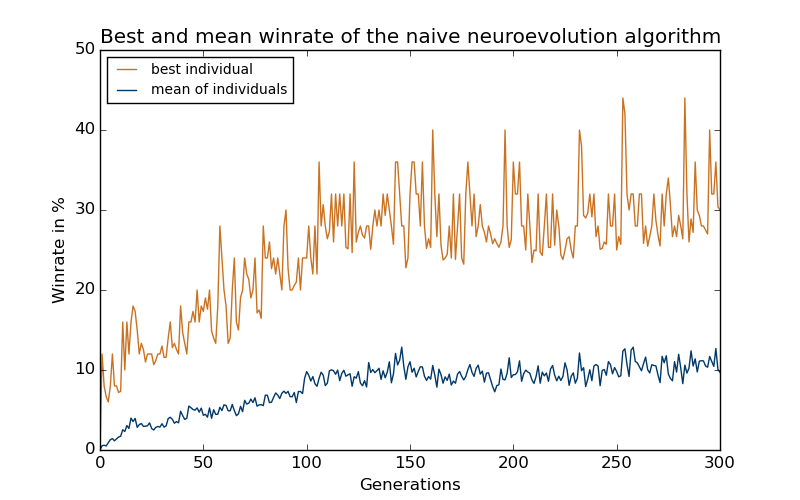
\includegraphics[scale=0.5]{../pictures/summary/neural-fitness.png}
                       \caption{Fitness Graph für Cross Entropy}\label{fig:graph-ne}
                    \end{figure}
                \end{multicols}

                \begin{table}[H]
                    \begin{center}
                    \begin{tabular}{ |l|r|r|r| } 
                        \hline
                        \hfill & Trained Fitness   & Tested Fitness  &          Error    \\ \hline
                          Nr.1 &          44.00\%  &         19.04\% &          56.72\%  \\  
                          Nr.2 &          44.00\%  &         20.18\% &          54.14\%  \\  
                          Nr.3 &          42.00\%  &         20.07\% &          52.21\%  \\ 
                          Nr.4 &          40.00\%  &         20.10\% &          49.75\%  \\ 
                          Nr.5 &          40.00\%  &         21.28\% &          46.80\%  \\ \hline
                          Mean &  \textbf{42.00\%} & \textbf{20.13\%} & \textbf{51.93\%}  \\ \hline
                    \end{tabular}
                    \end{center}
                    \caption{Stabilität der besten 5 Neurevolution Individuen \label{fig:neuroevotable}}
                \end{table}

                \noindent
                Die stabile Fitness ist bei knapp 20\% und damit gewinnen diese Individuen durchschnittliche jedes fünfte Spiel. Die Spielweise von diesem Ansatz könnte man \textit{geplant} erklären, da der Spieler oft zum Tor rennt, kurz vor dem Strafraum stehen bleibt und von Ecke zu Ecke pendelt bis er den Torwart etwas aus dem Tor gelockt hat um ein Tor zu schießen. Wenn er mal verliert, ist es weil er sofort zum Beginn des Spieles sich ins Aus schießt, oder zu nah am Tor ist, sodass ihm der Ball abgenommen wird.\\

                \begin{center} \textit{(Link zum Video)} \end{center}
\newpage
            \subsubsection*{CoSyNE}
%                ``Graph zeigen, Interpretation bzw. Erklärung''
                \begin{multicols}{2}
                    \noindent
                    \\[5mm]
                    Der CoSyNE Algorithmus ist in der durchschnittlichen Fitness knapp 5\% hinter der Neuroevolution, hat dafür aber ganze 15\% in der Stabilität verloren. Aus der Natur von dem CoSyNE gab es selbst bei der 300 Generation noch exterm unterschiedliche Individuen und eine Konvergenz war nicht zu erkennen. 
                    \begin{figure}[H]
                       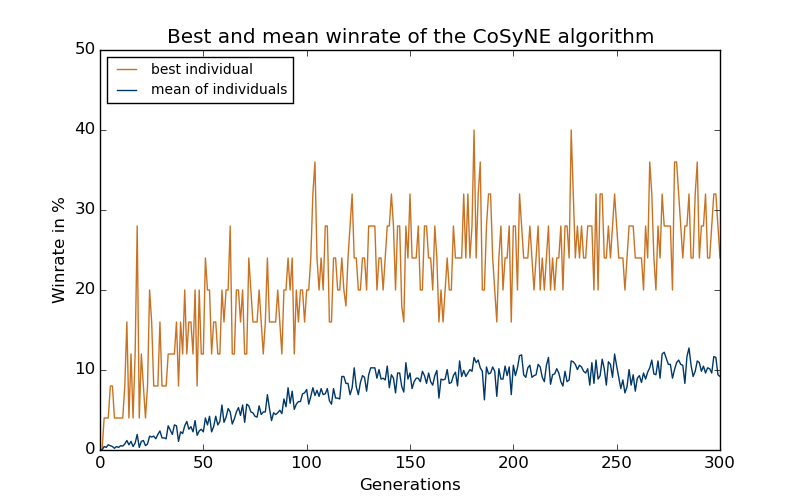
\includegraphics[scale=0.5]{../pictures/summary/cosyne-fitness.png}
                       \caption{Fitness Graph für Cross Entropy}\label{fig:graph-co}
                    \end{figure}
                \end{multicols}

                \begin{table}[H]
                    \begin{center}
                    \begin{tabular}{ |l|r|r|r| } 
                        \hline
                        \hfill & Trained Fitness   & Tested Fitness  &          Error    \\ \hline
                          Nr.1 &          40.00\%  &         14.21\% &          64.47\%  \\  
                          Nr.2 &          40.00\%  &         14.22\% &          64.45\%  \\  
                          Nr.3 &          36.00\%  &         12.68\% &          64.48\%  \\ 
                          Nr.4 &          36.00\%  &         15.42\% &          57.16\%  \\ 
                          Nr.5 &          36.00\%  &          5.75\% &          84.02\%  \\ \hline
                          Mean &  \textbf{37.60\%} & \textbf{12.45\%} & \textbf{66.98\%}  \\ \hline
                    \end{tabular}
                    \end{center}
                    \caption{Stabilität der besten 5 Neurevolution Individuen \label{fig:neuroevotable}}
                \end{table}
                \noindent
                Die beste Individuen haben lediglichlich nur knapp 12\% ihrer Spiele gewonnen und man kann eine ähnliche Taktik wie die Neuroevolution Agenten erahnen, nur wesentlich schlechter umgesetzt. Es passiert häufig, dass der Agent kurz vor dem Strafraum stehen bleibt und sich für eine sehr lange Zeit nicht bewegt. Da der Torwart nicht zu weit von dem Tor rausgeht, befinden sie sich im Deadlock bis der Agent versucht ein Tor zu schießen. Das Schießen am Anfang des Spiels tritt hier auf gehäuft auf.

                \begin{center} \textit{(Link zum Video)} \end{center}
\newpage
        \subsection{Vergleich}
%            ``Sicherheit <-> Aggressivität steht im Kontra zur Stabilität der Algorithmen''\\
%            ``Wenn Zeit ein Faktor wäre'' \\
%            ``Wenn Sicherheit ein Faktor wäre'' \\

             Im Vergleich zwischen allen Algorithmen sieht das Ranking folgendermaßen aus:

                \begin{table}[H]
                    \begin{center}
                    \begin{tabular}{ |l|r|r|r| } 
                        \hline
                        \textbf{Algorithmus}          & E(Trained Fitness) & E(Tested Fitness) & E(Error)    \\ \hline
                        Neuroevolution                &          42.00\%   &         20.13\%   &    51.93\%  \\ \hline
                        CoSyNE                        &          37.60\%   &         12.45\%   &    66.98\%  \\ \hline
                        Cross-Entropy                 &          29.60\%   &          6.56\%   &    77.87\%  \\ \hline
                        Wahrscheinlichkeitsverteilung &          24.60\%   &          6.15\%   &    74.88\%  \\ \hline
                    \end{tabular}
                    \end{center}
                    \caption{Alle Algorithmen gegenübergestellt \label{fig:vergleichstabelle}}
                \end{table}

            \noindent
            Neuroevolution gewinnt eindeutig in allen getesteten Merkmalen und hat während den Aufnahmen den raffiniertesten Eindruck gemacht. Wir sehen pauschale Aggressivität wie bei Cross-Entropy zwar interessante Züge macht, jedoch nicht tauglich ist für den Einsatz auf dem echten Spielfeld. \\[2mm]

            \noindent
            Sicherheit und die \textit{Planung} machen auf lange Sicht viel mehr Sinn und sollten verstärkt werden. Der CoSyNE Algorithmus unterstützt diese Art von Entwicklung in dieser Dimensionalität schlechter als die naive Suche über alle Parameter. Es ist zu überprüfen ob diese Aussage für gleichzeitiges Lernen in einem 2v1 Setting übereinstimmt.\\[2mm]

            \begin{center} \textit{(Link zur Best-Of-Compilation Video)} \end{center}